\documentclass[conference]{IEEEtran}
\IEEEoverridecommandlockouts

\usepackage{cite}
\usepackage{amsmath,amssymb,amsfonts}
\usepackage{graphicx}
\usepackage{booktabs}
\usepackage{xcolor}
\usepackage[hyphens]{url}
\usepackage[colorlinks=true,linkcolor=blue,citecolor=blue,urlcolor=blue]{hyperref}

\graphicspath{{../figures/}}

\begin{document}

\title{The Phenotype Definition Problem: How EHR Case Definitions Change the Genetic Overlap Between Autism and Its Co-occurring Medical Conditions}

\author{\IEEEauthorblockN{Kehinde Obidele}
\IEEEauthorblockA{\textit{Department of Health Informatics, Northeastern University}\\
ORCID: \href{https://orcid.org/0009-0008-6687-185X}{0009-0008-6687-185X}}}

\maketitle

\begin{abstract}
Genetic studies of medical conditions increasingly rely on case definitions written as rules over electronic health records, and a single condition often has several. This study asked how much the genetic correlation between autism and its co-occurring medical conditions moves when only that definition changes. Using public FinnGen R12 summary statistics for 28 endpoints, including alternative definitions of epilepsy, sleep apnoea, insomnia, constipation and ADHD, together with GWAS of autism (18,381 cases) and four larger psychiatric traits, we estimated 217 genetic correlations with LD score regression and built a block-jackknife test for the difference between two correlations that share a trait, on one common set of 953,474 SNPs. Every definition was also mapped to SNOMED CT through the OMOP standard vocabularies. Nine of 135 comparisons between definitions of the same condition survived Bonferroni correction. Widening sleep apnoea to any sleep disorder raised the genetic correlation with every psychiatric trait, by 0.03 to 0.07, and all functional bowel disorders correlated 0.21 more strongly with PTSD than constipation defined by diagnosis or laxative purchase, while adding primary care records moved it by 0.013 at most. For autism, no definition effect survived correction, and constipation gave the same correlation under both definitions (0.11 and 0.12) when a shift of 0.21 was detectable. Shared cases made differences precise: for nested definitions the smallest detectable shift fell to 0.015. The SNOMED CT mapping revealed that the constipation comparison was also a comparison of clinical scope, and distance in SNOMED CT tracked how far correlations moved (Spearman 0.49) better than overlap in codes and data sources did (0.13). How a condition is defined in the health record can change what genetics says about it, and the size of that change can be measured.
\end{abstract}

\begin{IEEEkeywords}
autism spectrum disorder, electronic health records, phenotype definition, genetic correlation, LD score regression, OMOP common data model, SNOMED CT, FinnGen, sleep, constipation, epilepsy
\end{IEEEkeywords}

\section{Introduction}
Autism rarely travels alone. Epilepsy is found in a median of 12.1\% of autistic people across 74 studies~\cite{lukmanji2019}, autistic children have almost four times the odds of constipation of comparison children~\cite{mcelhanon2014}, most experience sleep difficulties~\cite{richdale2009}, and incontinence is more common than in typically developing children~\cite{niemczyk2017}. For families these conditions are part of daily care, and earlier work on predicting toileting events for an autistic adult showed how much of that care revolves around the bladder and bowel~\cite{obidele2026toileting}. Twin and genome-wide studies suggest that part of this co-occurrence is shared genetic liability: in Swedish twins, clinical autism had genetic correlations of 0.50 with epilepsy and 0.31 with constipation~\cite{pan2023}, and genome-wide data give a genetic correlation of 0.27 between autism and irritable bowel syndrome~\cite{li2024}.

In biobank and health record studies, however, a condition is whatever its definition says it is. ``Constipation'' may mean a diagnosis code in a hospital record, a laxative purchase, or a wider group of functional bowel codes, and each rule captures different people. How much this matters shows up plainly in autism research: across 144 studies, the reported prevalence of constipation in autism ranged from 4.3\% to 45.5\%, and gastrointestinal symptoms differed significantly by how they were ascertained~\cite{holingue2018}. Phenotype libraries and electronic phenotyping methods exist to make definitions explicit and reusable~\cite{kirby2016,denaxas2019,banda2018}, yet one biobank can still publish several definitions of the same condition side by side.

The genetics of a condition can change with its definition. Depression defined by a few self-reported items has lower heritability and less specific genetic signal than strictly defined major depression~\cite{cai2020}; SNP heritability of bipolar disorder identified from health records ranged from 0.00 to 0.24 across four algorithms~\cite{chen2018}; and definitions of gout in the UK Biobank differed in heritability and in the number of associated variants they recovered~\cite{cadzow2017}. We found no study that asked the same question of autism's co-occurring medical conditions. This study measured how far the genetic correlation between autism, four other psychiatric traits and a set of medical conditions moves when only the case definition of the medical condition changes, and whether the answer is large enough to matter.

The study makes four contributions. It takes 28 FinnGen definitions apart into their codes, data sources and rules, and maps them to SNOMED CT through the OMOP standard vocabularies. It builds a difference test for two genetic correlations that share a trait, using LD score regression's own block jackknife on shared genome blocks, so that the correlation between the two estimates is part of the standard error. It reports, for every comparison, the smallest shift the data could have detected, so that a null result can be read as well powered or not. And it checks the method against a known definition effect, EHR against clinically defined depression.

\section{Related Work}

\subsection{Shared Genetics of Autism and Co-occurring Conditions}
Co-occurring psychiatric conditions in autism are well described, with pooled prevalence of 13\% for sleep-wake disorders and 28\% for ADHD~\cite{lai2019}. Genetic studies have mostly examined psychiatric and cognitive traits: a multivariate analysis of autism with eight co-occurring traits, all psychiatric or cognitive, identified shared loci and causal links~\cite{salenius2024}. Medical conditions have been studied less. The Swedish twin study found shared genetic effects between autism and epilepsy and gastrointestinal disorders across levels of symptom severity, but noted that without primary care records it probably captured only the more severe cases~\cite{pan2023}, which is itself a statement about definitions. Genome-wide work on functional somatic syndromes found positive genetic correlations of autism with irritable bowel syndrome, pain and fatigue~\cite{li2024}. Each of these studies used one definition per condition.

\subsection{Phenotype Definition and Genetic Signal}
Studies that vary a definition deliberately have focused on the condition being defined rather than on its genetic overlap with others. For depression, minimal phenotyping gave lower heritability and less specific loci than strict criteria~\cite{cai2020}, while 32 definitions built from diagnostic components in the UK Biobank had heritabilities from 0.102 to 0.162 and genetic correlations with external depression GWAS of 0.65 to 0.90, with no significant differences between the correlations~\cite{jermy2021}. EHR algorithms for bipolar disorder of different stringency correlated highly with conventionally ascertained cases~\cite{chen2018}, and gout definitions differed in heritability and power~\cite{cadzow2017}. None of these tested whether a definition change moves the genetic correlation with a second trait while accounting for the dependence between the estimates.

\subsection{EHR Phenotypes and Standard Vocabularies}
Rule-based EHR phenotypes are built mainly from diagnosis codes, then medications and text~\cite{kirby2016}, and platforms such as CALIBER curate validated definitions across several clinical terminologies~\cite{denaxas2019}. The OMOP common data model and its standard vocabularies let one definition be expressed once and run across health systems~\cite{overhage2012,hripcsak2015}. Phecodes group ICD codes into research phenotypes and have been mapped to WHO ICD-10~\cite{wu2019}, most recently as phecodeX~\cite{shuey2023}. This study uses both to compare definitions, and uses SNOMED CT as a measure of how different two definitions are in clinical meaning.

\subsection{Estimating Genetic Correlation}
LD score regression estimates heritability and genetic correlation from summary statistics and separates confounding and sample overlap into its intercept~\cite{bulik2015ldsc,bulik2015atlas}, and resources such as LD Hub made it routine to screen many traits~\cite{zheng2017}. Its estimates are less precise than those from individual-level methods, and less precise again when the reference LD panel does not match the study population~\cite{ni2018}. Genomic structural equation modelling uses the full sampling covariance of LD score regression estimates across traits~\cite{grotzinger2019}; this study uses the same idea, in its simplest form, to test differences between pairs of correlations.

\section{Methods}

\subsection{Study Design}
This study asked whether the genetic correlation between a psychiatric trait and a medical condition changes when only the electronic health record (EHR) definition of that condition changes (Fig.~\ref{fig:design}). It combined public summary statistics from the FinnGen biobank, which often publishes several definitions of the same condition, with genome-wide association studies (GWAS) of five psychiatric traits. Autism was the focal trait. Schizophrenia, bipolar disorder, major depression and post-traumatic stress disorder (PTSD) were added because their far larger samples make smaller definition effects detectable, and depression defined from EHRs and by clinical assessment served as a positive control where a definition effect is already known~\cite{cai2020}.

\subsection{Condition Definitions}
Condition GWAS came from FinnGen release R12 (500,348 participants)~\cite{kurki2023}. The endpoint definitions were taken from the R12 core and non-core endpoint file, which matches data freeze DF12, and were checked against the DF12 endpoint and control definition files (SHA-256 checksums recorded). A FinnGen endpoint is a set of rules: regular expressions over Finnish ICD-10, ICD-9 and ICD-8 codes in the hospital discharge and cause-of-death registers, optional codes from primary care (Avohilmo), drug purchase classes (ATC codes) and drug reimbursement rights, inclusion of other endpoints, exclusion conditions, a ``mode'' rule requiring the code to be the person's most frequent related diagnosis, and a separate rule for who may serve as a control.

This study grouped 28 endpoints. Eighteen formed six \emph{definition sets}, alternative definitions of one condition whose case groups overlap or nest: epilepsy (any epilepsy; focal, focal strict and focal mode; generalized, generalized strict and generalized mode), sleep apnoea (hospital records; hospital records plus primary care; any sleep disorder), insomnia (F51.0 or G47.0; all of F51 with stricter controls), constipation (the constipation code K59.0 or a laxative purchase; all functional intestinal disorders, K59), attention-deficit/hyperactivity disorder (F90.0; all of F90 with stricter controls) and intellectual disability (mild, F70; any, F7). Ten neighbouring conditions (for example irritable bowel syndrome, reflux and two bladder disorders) were analysed alongside for comparison. The grouping, and the choice of distance measure described below, were fixed in the study notebook before any genetic correlation was estimated. Two candidate groupings were rejected at that stage because their members shared no codes: the two bladder endpoints (N31 and N32) and the irritable bowel, dyspepsia and reflux endpoints are different conditions, not definitions of one.

Each definition was taken apart by a script that expanded every code pattern against the WHO ICD-10 code list, followed inclusion chains, and recorded which data sources and rules could make a person a case (Fig.~\ref{fig:anatomy}). Mild intellectual disability (913 cases) had a heritability estimate below zero and was excluded from all correlation analyses, which left five testable definition sets.

\subsection{Mapping to Standard Vocabularies}
To make definitions comparable across health systems, each definition's codes were mapped to the Observational Medical Outcomes Partnership (OMOP) standard vocabularies~\cite{hripcsak2015,overhage2012}, downloaded from Athena (WHO ICD-10 2021 release, ICD-9-CM, ATC 2026-02-01, SNOMED CT 2026 International edition, RxNorm 2026-06-01). ICD-10 codes were matched to OMOP ICD10 concepts and followed through the ``Maps to'' relationship to standard SNOMED CT concepts. Finnish ICD-9 codes, which add a letter to four digits, were matched to ICD-9-CM after removing the letter and are reported as approximate. ICD-8 has no OMOP vocabulary, so ICD-8 rules could not be mapped. ATC classes were linked to their substances through the concept ancestor table. The phecodeX map~\cite{shuey2023,wu2019} was used as a second, research-oriented grouping. The overlap between two definitions was measured with the Jaccard index at four levels: ICD-10 codes, phecodes, SNOMED CT concepts, and SNOMED CT concepts together with their ancestors up to two levels.

\subsection{Psychiatric GWAS}
Autism summary statistics came from the iPSYCH-PGC meta-analysis (18,381 cases, 27,969 controls)~\cite{grove2019}. The other psychiatric GWAS were the European-ancestry analyses of the Psychiatric Genomics Consortium for schizophrenia~\cite{trubetskoy2022}, bipolar disorder~\cite{mullins2021}, major depression excluding 23andMe~\cite{adams2025} and PTSD~\cite{nievergelt2024}, and the MDD2025 subsets restricted to EHR or registry cohorts (311,831 cases, 1,180,439 controls) and to clinically assessed cohorts (26,778 cases, 51,857 controls)~\cite{adams2025}. Per-SNP effective sample sizes were used for all PGC analyses. For every file, the reported frequency of the effect allele was compared with the 1000 Genomes European frequency of the same allele~\cite{kg2015}; correlations ranged from 0.991 to 0.998 over more than 1.1 million non-palindromic SNPs, confirming that effect alleles were labelled correctly.

The cohort lists showed three sources of sample overlap with FinnGen: the full depression GWAS and its EHR subset both include FinnGen, and the PTSD meta-analysis lists FinnGen among its biobanks. The EHR depression subset also contains iPSYCH, the cohort behind the autism GWAS. Cross-trait LD score regression absorbs such overlap in its intercept~\cite{bulik2015atlas}, and the intercepts were inspected for exactly this pattern.

\subsection{LD Score Regression}
SNP heritability and genetic correlation were estimated with LD score regression~\cite{bulik2015ldsc,bulik2015atlas} using a maintained Python 3 port of the original software and the European LD scores computed from 1000 Genomes~\cite{kg2015}. FinnGen files were streamed, restricted to HapMap3 SNPs with minor allele frequency of at least 0.01, and never stored; about 1.17 million SNPs remained per endpoint. Heritability was converted to the liability scale~\cite{lee2011}. For FinnGen endpoints the population prevalence was approximated by the sample prevalence, so heritability is compared within a condition rather than across conditions; genetic correlations do not depend on this choice.

Before any new estimate was trusted, the pipeline reproduced published values: autism liability-scale heritability 0.117 (SE 0.010) against 0.118 (SE 0.010) in the source paper~\cite{grove2019}, and the genetic correlation between autism and ADHD~\cite{demontis2019} of 0.346 (SE 0.051) against 0.360 (Fig.~\ref{fig:validation}). During this work a defect was found in the Python 3 port: requesting liability-scale output from a genetic correlation run raised an error after the estimate had been printed. Genetic correlations were therefore run without prevalence arguments, which leaves the estimate unchanged.

\subsection{Testing Whether the Definition Moves the Genetic Correlation}
Two genetic correlations that share a psychiatric trait and describe overlapping case groups have correlated sampling errors, and treating them as independent would overstate the uncertainty of their difference. LD score regression estimates standard errors with a block jackknife over 200 contiguous blocks of SNPs~\cite{busing1999}. All 35 traits were first restricted to one common set of 953,474 SNPs, and every pair was re-estimated with evenly spaced blocks, so that block $k$ covers the same stretch of genome in every analysis. From the delete values of the genetic covariance and the two heritabilities, the jackknife pseudovalue of the genetic correlation in block $k$ is
\begin{equation}
\tilde{r}_{k} = n\,\hat{r}_g - (n - 1)\,\frac{\hat{\rho}_{g,(k)}}{\sqrt{\hat{h}^2_{1,(k)}\,\hat{h}^2_{2,(k)}}},
\end{equation}
with $n = 200$, exactly as the software computes it. For two definitions $a$ and $b$, the standard error of the difference $\hat{r}_a - \hat{r}_b$ is $\sqrt{\mathrm{var}(\tilde{r}_{a,k} - \tilde{r}_{b,k})/n}$, which includes the covariance between the two estimates. The rebuilt standard error of every single genetic correlation matched the software's own printed value (198 of 198). The smallest difference detectable at a two-sided $\alpha$ of 0.05 with 80\% power is $2.80$ times this standard error.

Within each definition set and psychiatric trait, heterogeneity across all definitions was tested with Cochran's $Q = \hat{\mathbf{r}}^{\top} W \hat{\mathbf{r}} - (\mathbf{1}^{\top} W \hat{\mathbf{r}})^2 / (\mathbf{1}^{\top} W \mathbf{1})$, where $W$ is the inverse of the jackknife covariance matrix of the definitions' estimates, on $k - 1$ degrees of freedom. The relation between how different two definitions are and how far their genetic correlations move was examined with Spearman correlations against the pre-specified distance (one minus the mean of ICD-10 Jaccard, data-source Jaccard and an indicator that no rule differs) and, as an exploratory analysis, against SNOMED CT distance. Because comparisons share traits and definitions, these correlations are descriptive.

\subsection{Finnish Linkage Disequilibrium}
The European LD reference does not match the Finnish population exactly~\cite{lim2014}. As a sensitivity check, LD scores were rebuilt for chromosomes 21 and 22 from the public FinnGen R12 LD matrix (520,210 samples; all variant pairs within 3 Mb with $r^2 > 0.01$), summing $r^2$ over HapMap3 SNPs within 1 Mb, and compared SNP by SNP with the European scores.

\section{Results}

\begin{figure*}[t]
\centering
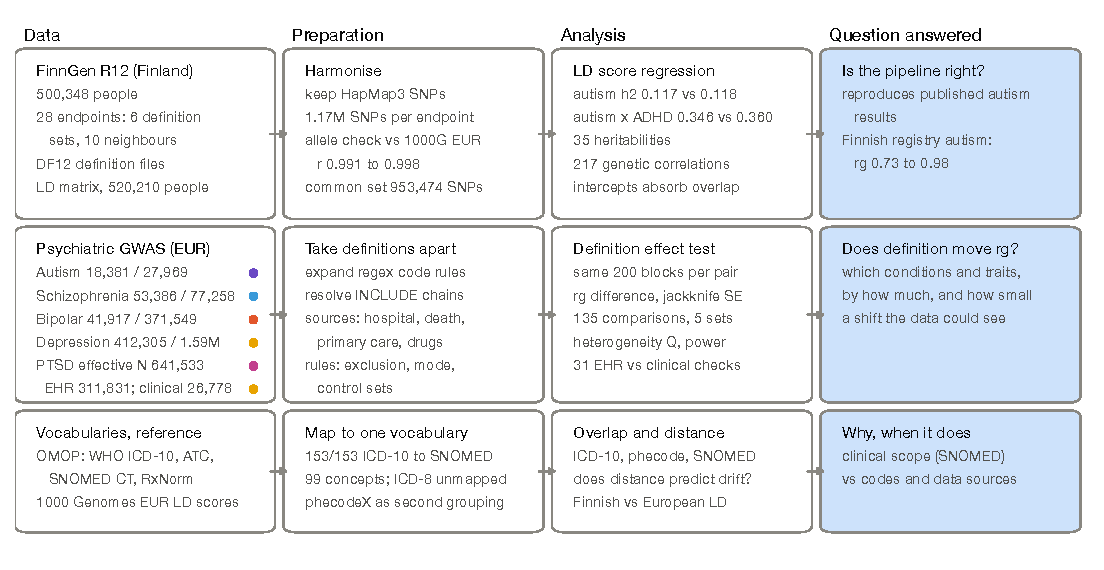
\includegraphics[width=\textwidth]{fig01_design.pdf}
\caption{Study design. Data came from FinnGen R12 (definitions and summary statistics), five European-ancestry psychiatric GWAS with EHR and clinical depression subsets, and the OMOP vocabularies. Each row follows one strand from preparation to analysis to the question it answers. Every count is taken from this study's files and logs.}
\label{fig:design}
\end{figure*}

\subsection{What the Definitions Contain}
Alternative definitions of the same condition differed in several ways at once (Fig.~\ref{fig:anatomy}). Some shared every ICD-10 code and differed only in their rules: focal, focal strict and focal mode epilepsy all use G40.0 to G40.2, but the strict version excludes anyone who also meets the generalized definition and the mode version requires focal codes to be the person's most frequent epilepsy diagnosis. Others differed in their data sources: the two sleep apnoea definitions share one code (G47.3), and the broader one adds primary care records. The constipation definition counts a laxative purchase as a case, which no code-based view can show.

\begin{figure*}[t]
\centering
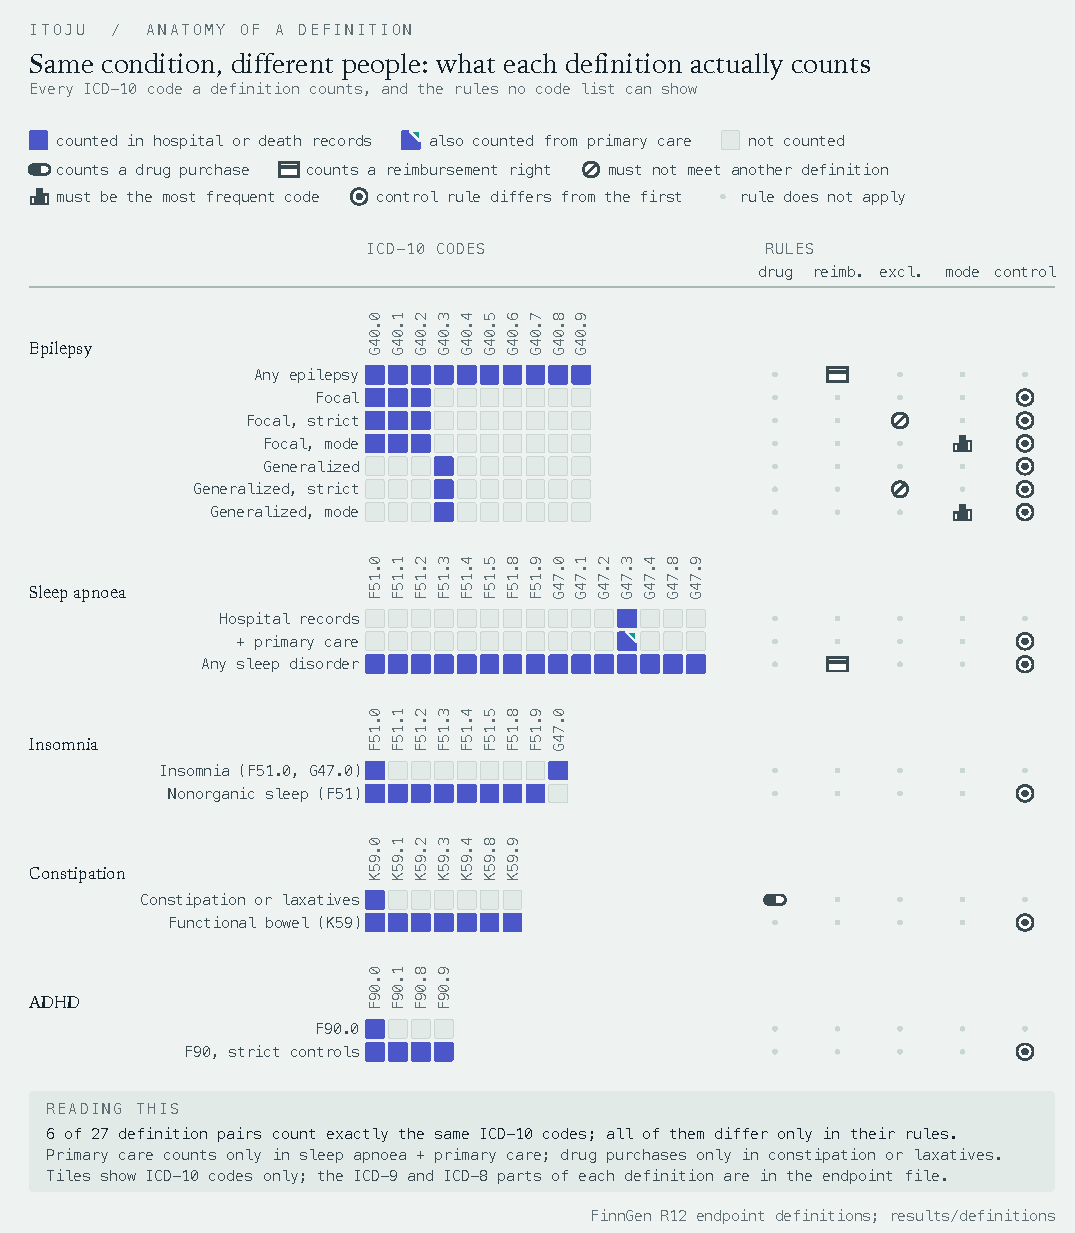
\includegraphics[width=\textwidth]{fig02_anatomy.pdf}
\caption{The anatomy of a definition. Each row is one alternative definition. Left block: one column per ICD-10 code used anywhere in that condition's definitions; a filled tile means the code makes someone a case in hospital or death records, and a white notch marks codes also counted from primary care. Right block: rules that codes cannot show. drug, a drug purchase class counts (ATC A06A, laxatives); reimb, a drug reimbursement right counts; excl, a case must not also meet another definition; mode, the code must be the most frequent related diagnosis; ctrl, the control rule differs from the first definition in the set. Tiles show ICD-10 only.}
\label{fig:anatomy}
\end{figure*}

All 153 ICD-10 codes used across the 28 definitions mapped to standard SNOMED CT concepts (99 distinct concepts). Sixteen of the 28 definitions also contain ICD-8 rules, which have no OMOP counterpart. How much two definitions overlapped depended on the vocabulary used to compare them (Fig.~\ref{fig:lenses}). Attention-deficit/hyperactivity disorder defined as F90.0 or as all of F90 overlapped 0.20 by ICD-10 codes, 1.00 by phecodes, 0.50 by SNOMED CT concepts and 0.80 once SNOMED CT ancestors were included. Any epilepsy and generalized epilepsy overlapped 0.09 by codes but 0.50 in the SNOMED CT hierarchy. The two bladder endpoints shared no codes and no phecodes but 28\% of their SNOMED CT concepts.

\begin{figure}[t]
\centering
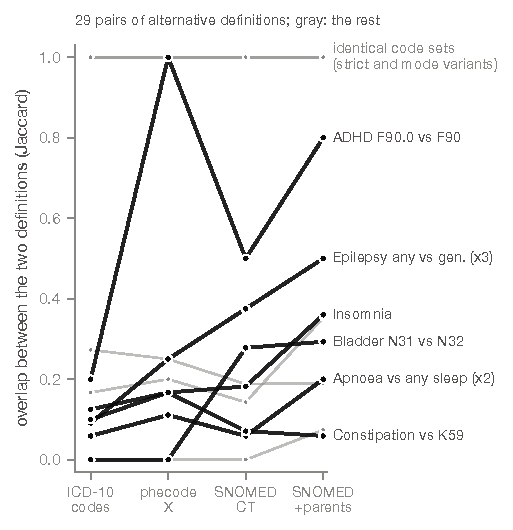
\includegraphics[width=\columnwidth]{fig05_three_lenses.pdf}
\caption{Three lenses on overlap. For each pair of alternative definitions, the Jaccard overlap measured from ICD-10 codes, phecodeX groups, SNOMED CT concepts, and SNOMED CT concepts together with their ancestors within two levels. Black lines are named pairs; gray lines are the remaining pairs; ``x3'' marks identical profiles merged. The flat line at 1.0 is the strict and mode variants, whose code sets are identical.}
\label{fig:lenses}
\end{figure}

Reading the definitions through SNOMED CT also caught a labelling error in this study's own work (Fig.~\ref{fig:snomed}). The FinnGen endpoint first treated here as a diagnosis-only definition of constipation (K59) maps to 14 SNOMED CT concepts: constipation and its subtypes, but also irritable bowel syndrome, functional diarrhoea, neurogenic bowel, acquired megacolon and post-surgical conditions. FinnGen's own name for it is ``other functional intestinal disorders''. It is a broader bowel dysfunction definition that contains constipation, and it is described as such throughout. In the same way, insomnia defined by F51.0 or G47.0 maps to two concepts, while all of F51 adds sleepwalking, sleep terrors, nightmares, non-organic hypersomnia and sleep-wake schedule disorders (11 concepts).

\begin{figure}[t]
\centering
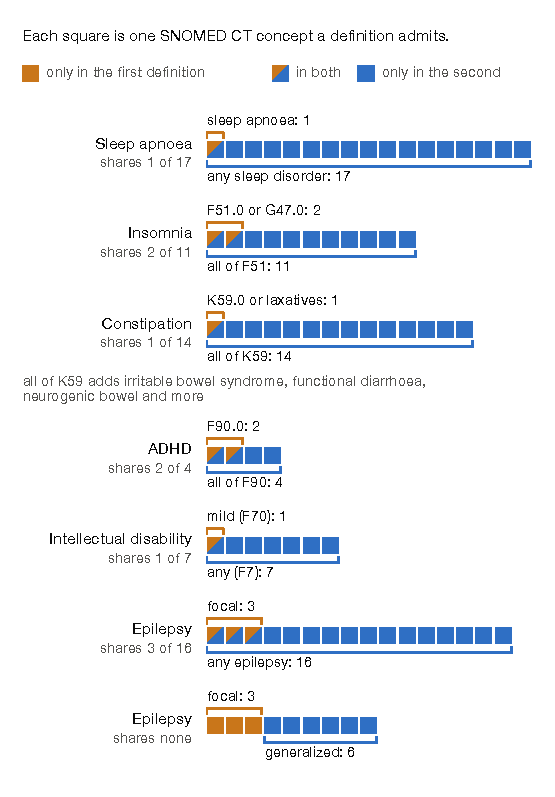
\includegraphics[width=\columnwidth]{fig06_snomed_contents.pdf}
\caption{What a definition contains, read in SNOMED CT. Rows are the standard concepts that each definition's ICD-10 codes map to; a filled dot means the definition includes the concept. (a) Insomnia, (b) constipation against all functional intestinal disorders (K59), (c) ADHD. Concepts in both definitions are in darker text.}
\label{fig:snomed}
\end{figure}

\subsection{Validation, Heritability and Genetic Correlations}
The pipeline reproduced the published autism estimates before any new result was produced (Fig.~\ref{fig:validation}). Autism in the Danish GWAS also correlated strongly with autism in the Finnish registry: $r_g = 0.73$ (SE 0.15) with the narrow FinnGen definition (F84.0, F84.5; 888 cases) and 0.98 (SE 0.21) with the broader one (F84; 1,179 cases).

\begin{figure*}[t]
\centering
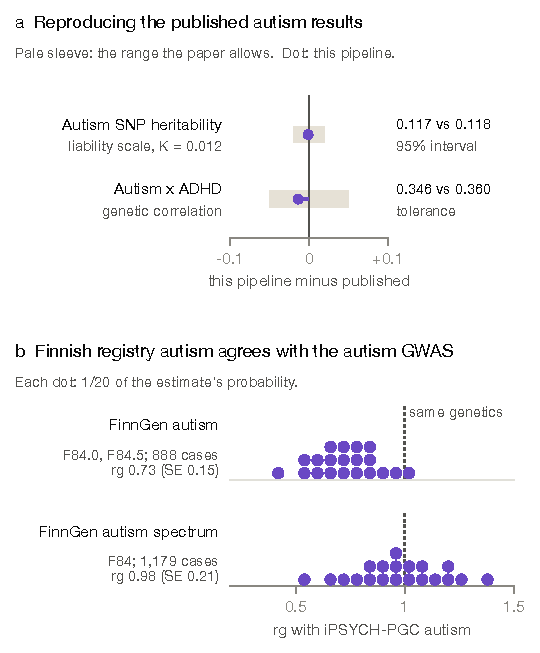
\includegraphics[width=\textwidth]{fig07_validation.pdf}
\caption{Validation. (a) Autism SNP heritability on the liability scale and the genetic correlation between autism and ADHD, from this pipeline (filled, 95\% interval) and as published (hollow; the published correlation has no printed standard error). (b) Genetic correlation between the iPSYCH-PGC autism GWAS and the two FinnGen autism endpoints.}
\label{fig:validation}
\end{figure*}

Liability-scale heritability varied within conditions (Fig.~\ref{fig:h2}). Generalized epilepsy (0.135, SE 0.032) was more heritable than focal epilepsy (0.026, SE 0.009), and the broad epilepsy definition fell between them (0.055, SE 0.009). ADHD with all of F90 and stricter controls (0.127, SE 0.019) exceeded F90.0 alone (0.092, SE 0.016). Adding primary care to sleep apnoea left heritability unchanged (0.125 and 0.120). Among the psychiatric traits, clinically defined depression had twice the heritability of EHR-defined depression (0.114, SE 0.012, against 0.057, SE 0.002, at the same population prevalence), the direction reported for strict versus minimal definitions of depression~\cite{cai2020}. Mild intellectual disability (913 cases) had an estimate below zero.

\begin{figure}[t]
\centering
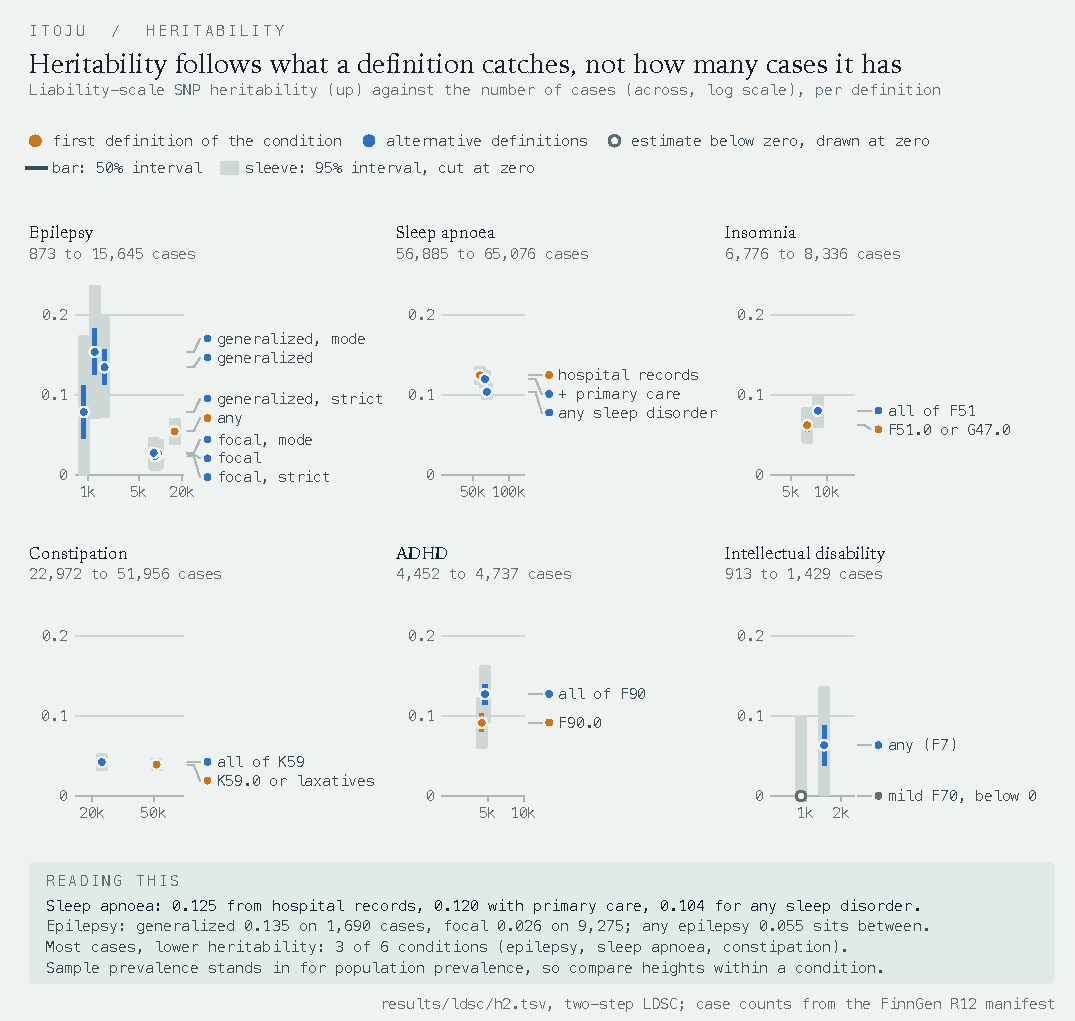
\includegraphics[width=\columnwidth]{fig08_heritability.pdf}
\caption{SNP heritability by definition. Left: liability-scale heritability with 95\% interval, using the sample prevalence as the population prevalence. Right: number of cases, log scale. A hollow mark at zero is an estimate below zero.}
\label{fig:h2}
\end{figure}

Of the 217 genetic correlations estimated, 156 had $p < 0.05$ (Fig.~\ref{fig:quilt}). The genetic correlation between schizophrenia and bipolar disorder was 0.68 (SE 0.02). Autism correlated with both FinnGen ADHD definitions (0.53, SE 0.11; 0.55, SE 0.08), irritable bowel syndrome (0.22, SE 0.07), nonorganic sleep disorders (0.31, SE 0.09) and sleep apnoea (0.12, SE 0.05), but not with any epilepsy definition (estimates from $-0.19$ to $-0.02$). The cross-trait intercepts behaved as expected from the cohort lists (Fig.~\ref{fig:intercepts}): median 0.001 to 0.004 for autism, schizophrenia, bipolar disorder and clinical depression, which contain no FinnGen samples, against 0.012 for PTSD and 0.020 for both depression GWAS that include FinnGen.

\begin{figure}[t]
\centering
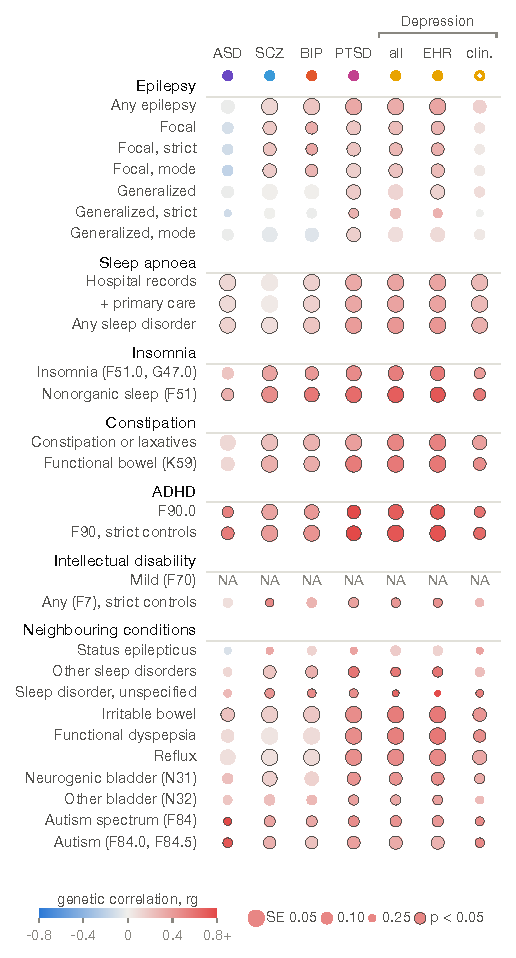
\includegraphics[width=\columnwidth]{fig09_rg_quilt.pdf}
\caption{Genetic correlations between seven psychiatric GWAS and 28 FinnGen endpoints. Dot color is $r_g$ (capped at $\pm 0.8$); dot area grows with precision, so estimates with wide standard errors shrink; a gray ring marks $p < 0.05$. NA: heritability below zero. Rows are grouped by condition, with the definitions of one condition stacked together.}
\label{fig:quilt}
\end{figure}

\begin{figure}[t]
\centering
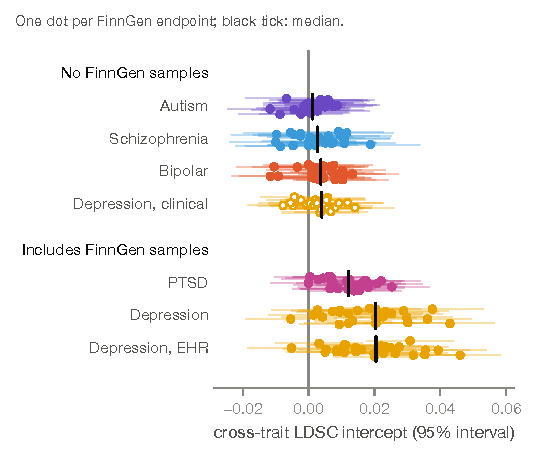
\includegraphics[width=\columnwidth]{fig18_intercepts.pdf}
\caption{Cross-trait LD score regression intercepts with the 28 FinnGen endpoints, grouped by whether the psychiatric GWAS contains FinnGen samples. One dot per endpoint with 95\% interval; black tick, median. Shared samples appear in the intercept, which keeps $r_g$ unbiased.}
\label{fig:intercepts}
\end{figure}

\subsection{Does the Definition Move the Genetic Correlation?}
All 198 estimable correlations were re-estimated on the common SNP set with shared jackknife blocks; they correlated 0.991 with the standard estimates (mean absolute difference 0.020). Across 135 comparisons between definitions of the same condition, 40 differences had $p < 0.05$ and nine survived Bonferroni correction ($p < 0.00037$). Table~\ref{tab:q} summarises heterogeneity across all definitions in each set, and Fig.~\ref{fig:sizing} shows every estimate against the smallest shift the design could detect.

\begin{table}[t]
\caption{Heterogeneity of genetic correlation across definitions of the same condition}
\label{tab:q}
\centering
\small
\begin{tabular}{@{}lccccc@{}}
\toprule
Set (definitions) & ASD & SCZ & BIP & MDD & PTSD \\
\midrule
Sleep apnoea (3) & 5.8 & 40.6$^{\ast}$ & 51.7$^{\ast}$ & 87.6$^{\ast}$ & 69.5$^{\ast}$ \\
Insomnia (2) & 3.1 & 4.8$^{\dagger}$ & 7.7$^{\dagger}$ & 7.7$^{\dagger}$ & 6.2$^{\dagger}$ \\
Constipation (2) & 0.0 & 5.9$^{\dagger}$ & 1.2 & 2.8 & 14.0$^{\ast}$ \\
ADHD (2) & 0.1 & 2.2 & 0.5 & 0.0 & 0.0 \\
Epilepsy (7) & 6.1 & 8.0 & 16.4$^{\dagger}$ & 21.0$^{\dagger}$ & 19.8$^{\dagger}$ \\
\bottomrule
\end{tabular}
\\[2pt]
\footnotesize{Cochran's $Q$ with the jackknife covariance, df = definitions $-$ 1. $^{\dagger}p < 0.05$; $^{\ast}p < 0.001$.}
\end{table}

\begin{figure*}[t]
\centering
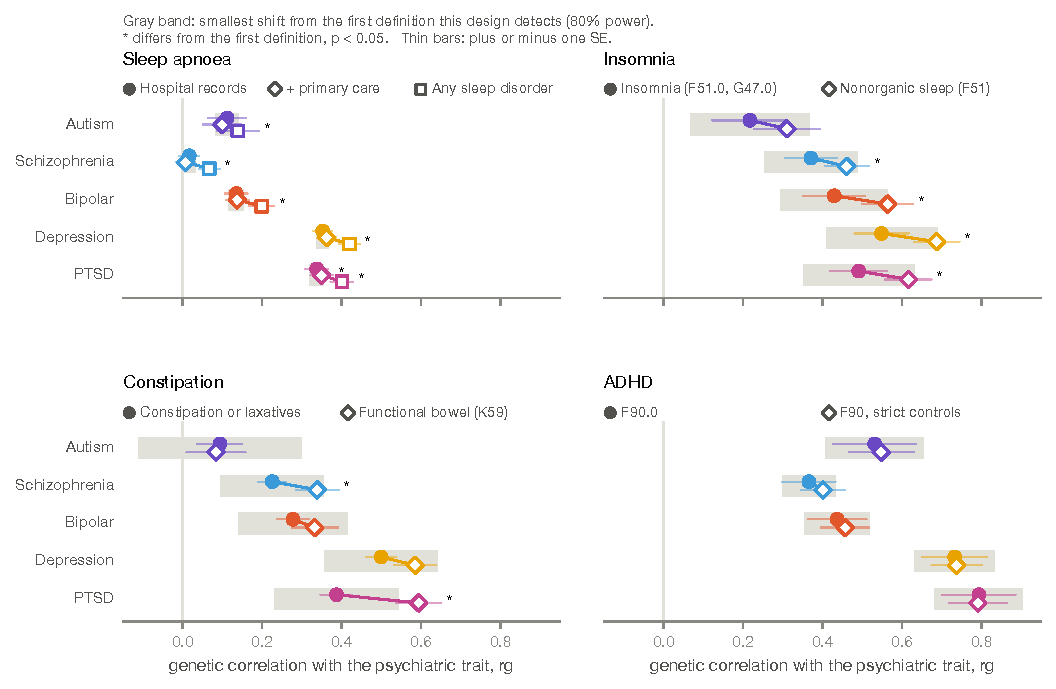
\includegraphics[width=\textwidth]{fig10_sizing_strips.pdf}
\caption{The same condition measured through different definitions. For each definition set and psychiatric trait, every definition's $r_g$ on one axis, joined by a line; thin bars, $\pm 1$ SE. The gray band spans the smallest shift from the first definition this design detects at 80\% power. $\ast$, the definition differs from the first definition at $p < 0.05$.}
\label{fig:sizing}
\end{figure*}

\emph{Sleep apnoea.} Adding primary care records barely moved the genetic correlation: the largest difference was 0.013 (SE 0.006, $p = 0.04$, PTSD), and the smallest detectable differences for this pair were 0.015 to 0.029. Widening the definition from sleep apnoea to any sleep disorder raised the genetic correlation with every psychiatric trait: by 0.068 (SE 0.007) for depression, 0.064 (SE 0.009) for bipolar disorder, 0.063 (SE 0.008) for PTSD, 0.050 (SE 0.008) for schizophrenia and 0.027 (SE 0.013, $p = 0.042$) for autism. These were the most precise comparisons in the study because the two definitions share most of their cases: their sampling errors correlated 0.92 to 0.97 (Fig.~\ref{fig:pseudo}).

\begin{figure*}[t]
\centering
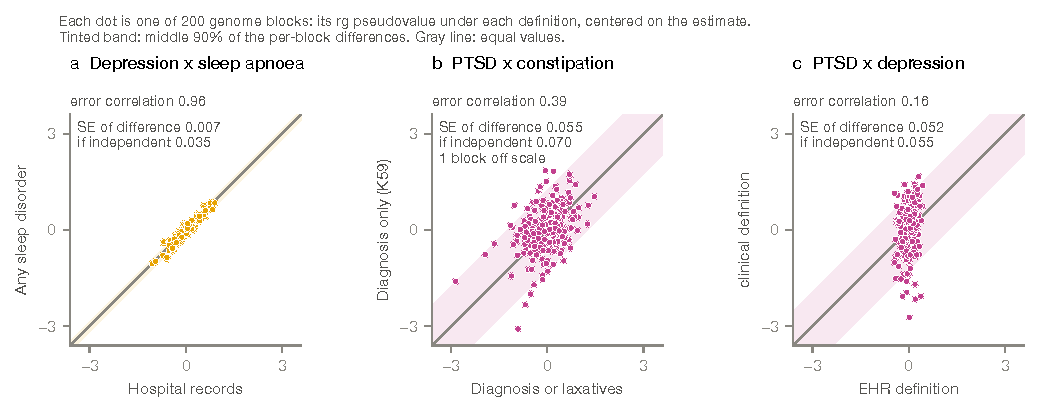
\includegraphics[width=\textwidth]{fig11_pseudovalues.pdf}
\caption{Why a difference between two genetic correlations can be precise. Each dot is one of 200 genome blocks: its jackknife pseudovalue of $r_g$ under each definition, centered on the estimate. When definitions share their cases, the blocks fall along the diagonal and most noise cancels in the difference. (a) Depression with sleep apnoea against any sleep disorder, (b) PTSD with constipation against functional intestinal disorders, (c) PTSD with EHR against clinical depression.}
\label{fig:pseudo}
\end{figure*}

\emph{Insomnia.} Nonorganic sleep disorders (all of F51, stricter controls) gave higher genetic correlations than insomnia (F51.0 or G47.0) for all five traits: by 0.139 (SE 0.050, $p = 0.005$) for depression, 0.134 (SE 0.048, $p = 0.005$) for bipolar disorder, 0.125 (SE 0.050, $p = 0.013$) for PTSD, 0.090 (SE 0.041, $p = 0.029$) for schizophrenia and 0.093 ($p = 0.079$) for autism. The two definitions differ in scope (parasomnias and hypersomnia added) and in their control rule at the same time, and this design cannot separate the two.

\emph{Constipation.} The broader functional intestinal disorders definition gave a higher genetic correlation than the constipation code or laxative definition for PTSD (0.207, SE 0.055, $p = 0.0002$) and schizophrenia (0.113, SE 0.046, $p = 0.015$), but not for autism (0.010, $p = 0.90$). The error correlation for this pair was only 0.39 to 0.55, because the laxative rule adds many people the diagnosis-based definition does not contain, so the smallest detectable differences were 0.13 to 0.21.

\emph{Epilepsy and ADHD.} Genetic correlations differed across the seven epilepsy definitions for depression ($Q = 21.0$, df 6, $p = 0.002$), PTSD ($p = 0.003$) and bipolar disorder ($p = 0.012$). The differences ran between focal and generalized epilepsy, not between strict, mode and plain versions of the same subtype. Both ADHD definitions gave the same correlations with every trait (largest difference 0.036), with smallest detectable differences of 0.07 to 0.12.

\begin{figure*}[t]
\centering
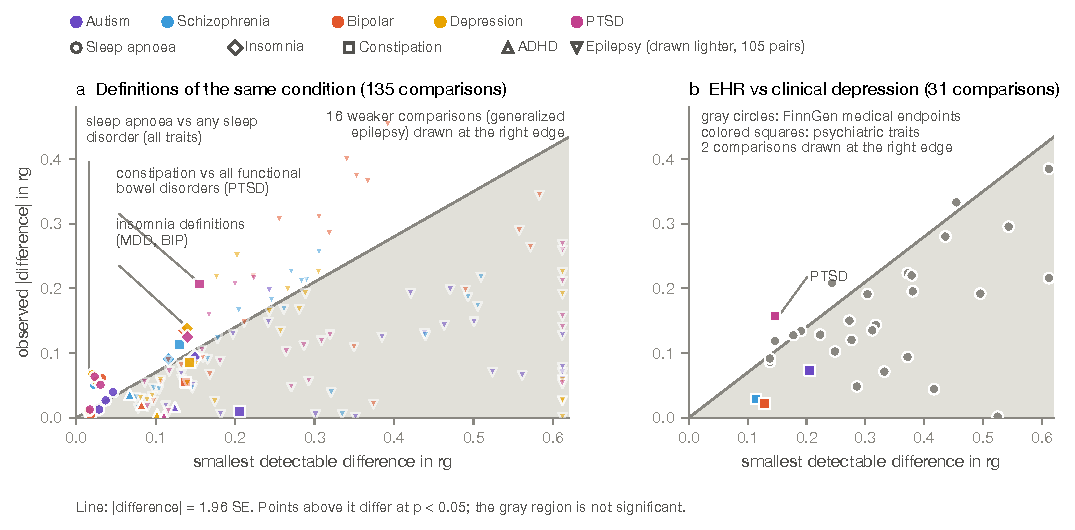
\includegraphics[width=\textwidth]{fig12_detectability.pdf}
\caption{Every comparison against its own power. The horizontal axis is the smallest difference each comparison could detect (80\% power); the vertical axis is the observed difference. Points above the line differ at $p < 0.05$. (a) The 135 comparisons between definitions of the same condition, colored by psychiatric trait and shaped by condition; epilepsy points are drawn lighter because they are numerous. (b) The 31 comparisons between EHR and clinical depression.}
\label{fig:detect}
\end{figure*}

\begin{figure}[t]
\centering
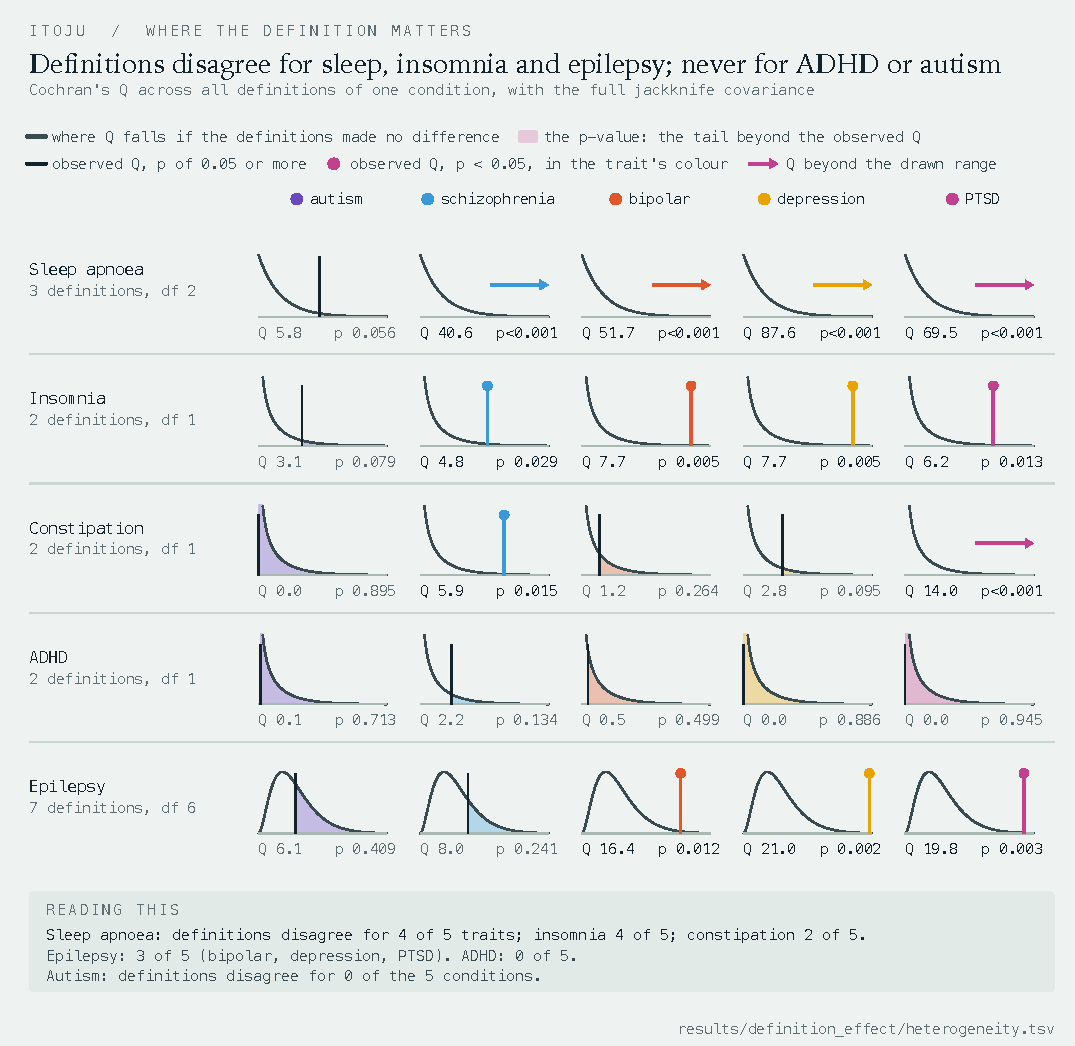
\includegraphics[width=\columnwidth]{fig13_heterogeneity.pdf}
\caption{Heterogeneity across definitions. Rows, definition sets; columns, psychiatric traits. Dot fill is $-\log_{10} p$ of Cochran's $Q$ (capped at 8), dot size the range of $r_g$ across definitions, and a ring marks $p < 0.05$, labelled with $Q$ and its degrees of freedom.}
\label{fig:hetero}
\end{figure}

\begin{figure}[t]
\centering
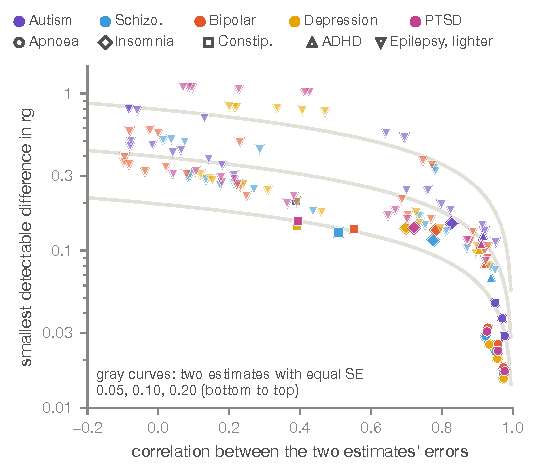
\includegraphics[width=\columnwidth]{fig20_power.pdf}
\caption{What buys power: shared cases. Smallest detectable difference in $r_g$ against the correlation between the two estimates' sampling errors, for all 135 comparisons. Gray curves show the formula for two estimates with equal standard errors of 0.05, 0.10 and 0.20.}
\label{fig:power}
\end{figure}

Across all 135 comparisons, the smallest detectable difference ranged from 0.015 to 1.10 (Fig.~\ref{fig:detect}), and it was governed mainly by how strongly the two estimates' errors correlated (Fig.~\ref{fig:power}).

\subsection{Autism}
For autism, no difference between definitions survived multiple-testing correction (Fig.~\ref{fig:autism}). Three were nominally significant: widening sleep apnoea to any sleep disorder, from hospital records (0.027, $p = 0.042$) and from hospital plus primary care records (0.040, $p = 0.017$), in the same direction as for every other trait, and any epilepsy against focal epilepsy under the mode rule (0.197, $p = 0.023$). The design could see a shift of 0.03 to 0.05 for the sleep apnoea definitions, 0.15 for insomnia, 0.21 for constipation and 0.12 for ADHD, but between 0.11 and 0.81 for epilepsy. The constipation result is the clearest statement for autism: whether the definition is narrow constipation or all functional bowel disorders, the genetic correlation with autism is the same (0.11 and 0.12).

\begin{figure}[t]
\centering
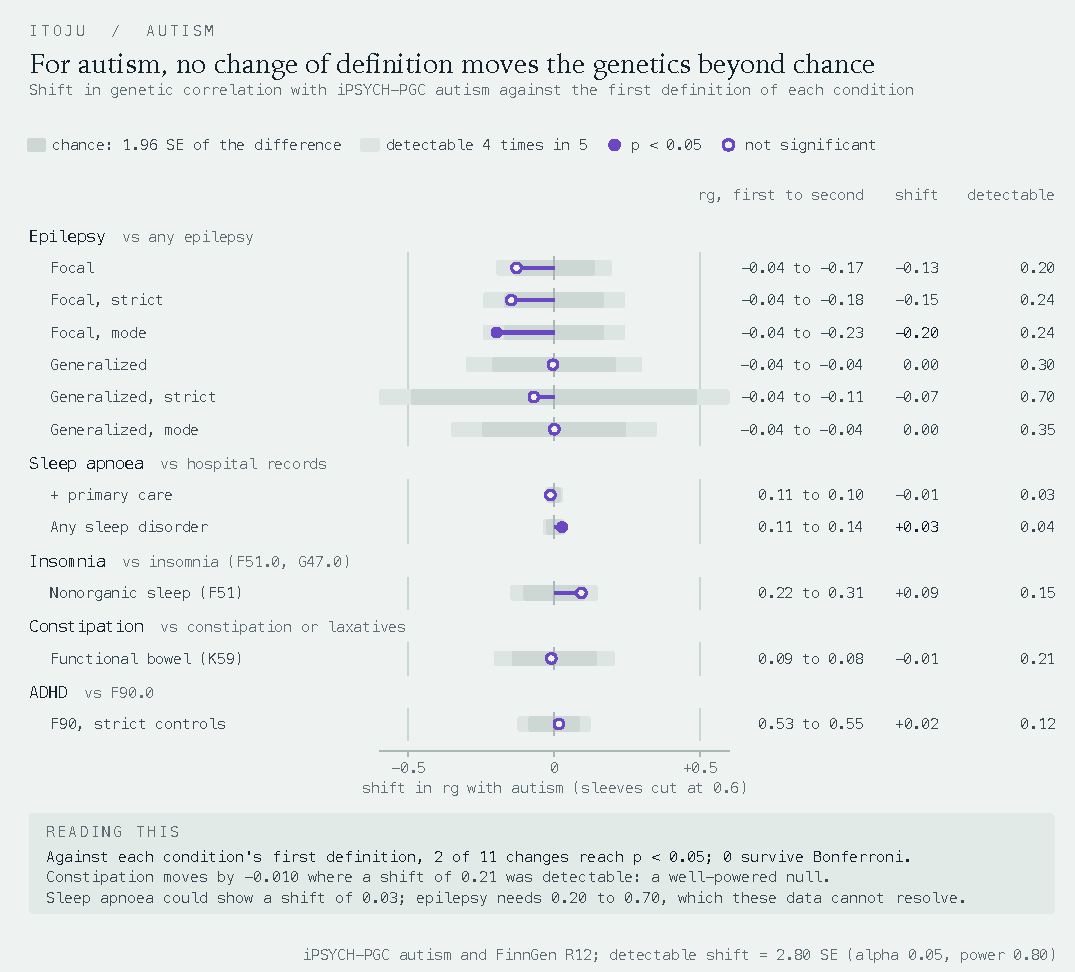
\includegraphics[width=\columnwidth]{fig16_autism_focus.pdf}
\caption{Autism in focus. Left: $r_g$ with iPSYCH-PGC autism and 95\% interval for every definition. Right: the shift from the first definition in each condition, drawn against the smallest shift detectable at 80\% power (gray bar); a ringed dot differs at $p < 0.05$.}
\label{fig:autism}
\end{figure}

\subsection{Positive Control: EHR and Clinical Depression}
EHR-defined and clinically defined depression correlated at $r_g = 0.857$ (SE 0.045). Against the other traits and endpoints, EHR depression gave the higher genetic correlation in 25 of 31 comparisons (Fig.~\ref{fig:control}); six differences had $p < 0.05$ and none survived Bonferroni correction. The largest were with PTSD (0.157, SE 0.052, $p = 0.003$) and any epilepsy (0.208, $p = 0.017$). Because the two depression GWAS share almost no samples (intercept 0.013), their errors were only weakly correlated, and the smallest detectable differences were 0.11 to 1.19.

\begin{figure}[t]
\centering
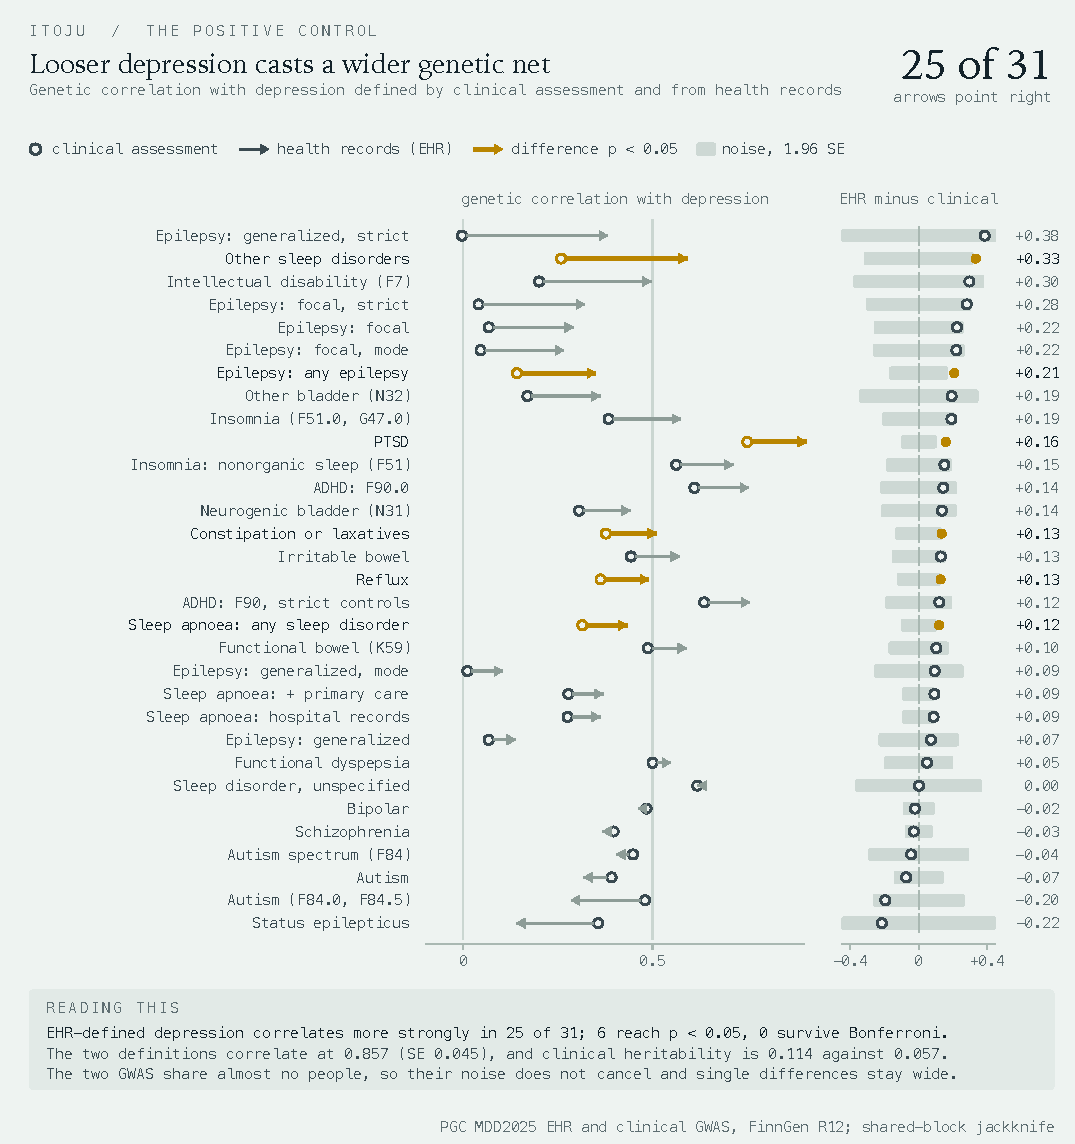
\includegraphics[width=\columnwidth]{fig15_positive_control.pdf}
\caption{Positive control. For every other trait and FinnGen endpoint, $r_g$ with EHR-defined depression (filled) and with clinically defined depression (hollow). $\ast$, the difference is significant at $p < 0.05$ by the jackknife test.}
\label{fig:control}
\end{figure}

\subsection{Distance Between Definitions}
The pre-specified definition distance, built from shared codes, data sources and rules, did not predict how far the genetic correlation moved (Spearman $\rho = 0.13$ across all comparisons; Fig.~\ref{fig:distance}). Distance in SNOMED CT did ($\rho = 0.49$; 0.84 for schizophrenia, 0.66 for bipolar disorder, 0.54 for autism), an exploratory result carried mostly by the epilepsy comparisons, which make up 105 of the 135.

\begin{figure*}[t]
\centering
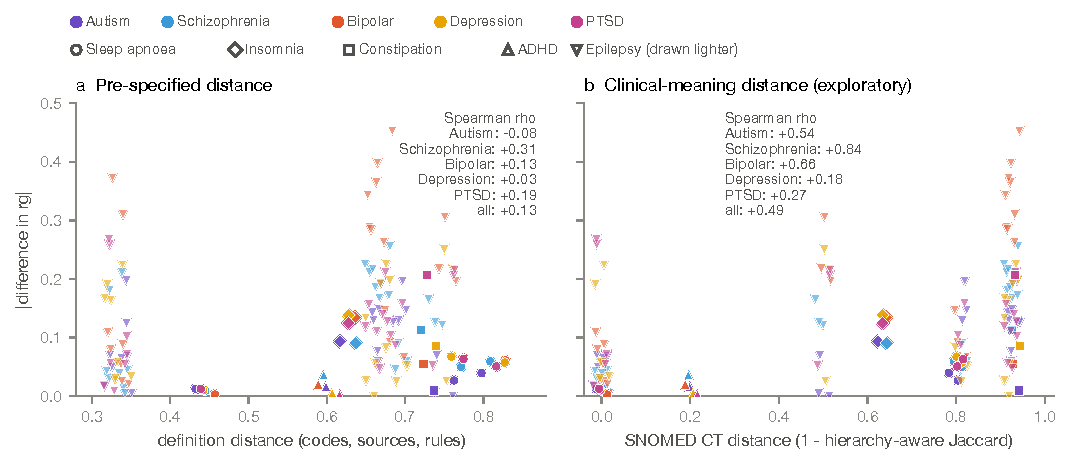
\includegraphics[width=\textwidth]{fig14_distance_drift.pdf}
\caption{Do definitions that differ more give genetic correlations that differ more? Each point is one comparison. (a) Pre-specified distance from codes, data sources and rules. (b) SNOMED CT distance (exploratory). Spearman correlations are descriptive because comparisons share traits and definitions.}
\label{fig:distance}
\end{figure*}

\subsection{Finnish Linkage Disequilibrium}
On chromosomes 21 and 22, Finnish LD scores built from the FinnGen LD matrix correlated 0.970 with the European reference across 33,436 HapMap3 SNPs, with a median Finnish-to-European ratio of 1.009 (Fig.~\ref{fig:finnish}).

\begin{figure*}[t]
\centering
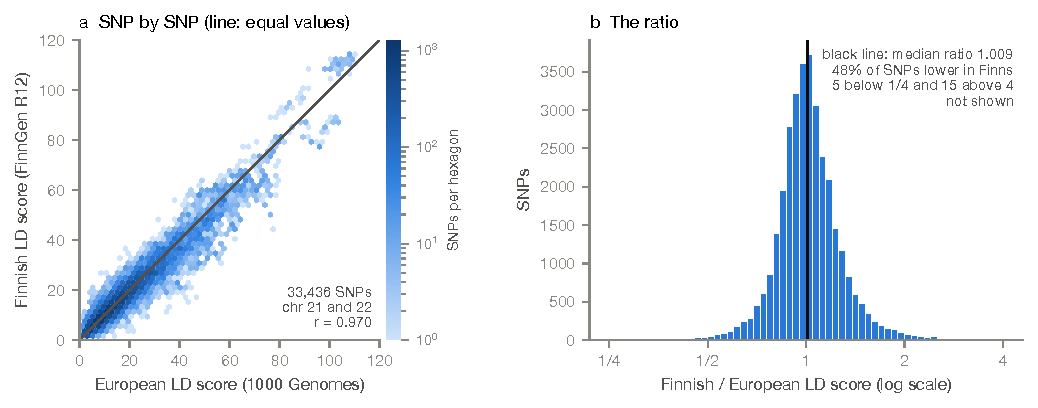
\includegraphics[width=\textwidth]{fig19_finnish_ld.pdf}
\caption{Finnish against European LD scores on chromosomes 21 and 22. (a) Log-density hexbin, one SNP per point, with the line of equality. (b) Distribution of the per-SNP ratio of Finnish to European LD score on a log axis.}
\label{fig:finnish}
\end{figure*}

\section{Discussion}

\subsection{What a Definition Changes, and What It Does Not}
The clearest pattern in these results is that the scope of a definition moved the genetic correlation, while the source of the records and the strictness of the rules mostly did not. Adding primary care records to sleep apnoea added nearly 6,000 cases and changed no correlation by more than 0.013, a null that the design could see down to 0.015. Strict and mode versions of focal and generalized epilepsy agreed closely with their plain versions. By contrast, widening sleep apnoea to any sleep disorder, which brings in insomnia, narcolepsy and other sleep diagnoses, raised the correlation with every psychiatric trait; moving from insomnia to all nonorganic sleep disorders raised it for all five; and moving from constipation to all functional bowel disorders raised it for PTSD and schizophrenia. In each case the wider definition added conditions that themselves carry psychiatric liability. Epilepsy followed the same logic from the other side: focal and generalized epilepsy, which have partly distinct genetic bases~\cite{ilae2018}, gave different correlations, and the broad definition fell between them.

This is why SNOMED CT distance tracked the size of the shift better than the pre-specified distance built from codes and data sources. The pre-specified measure counted differences, such as a primary care source or a stricter control rule, that turned out not to matter, and treated a subtype change as no larger than those. Distance in clinical meaning is a better guide to whether two definitions will give different genetics, although this finding is exploratory and rests mostly on the epilepsy comparisons.

The SNOMED CT view was also how this study caught its own mistake. A definition first treated as diagnosis-only constipation turned out to be all functional intestinal disorders, including irritable bowel syndrome and functional diarrhoea. Codes that read as a single condition can hide a much wider clinical scope, and mapping a definition to a standard vocabulary before using it is a cheap way to see that.

\subsection{Autism}
For autism the answer was reassuring rather than dramatic. No definition effect survived correction. The genetic correlation between autism and bowel dysfunction was the same whether the net was narrow constipation or all functional bowel disorders (0.11 and 0.12), with a detectable shift of 0.21, and the sleep apnoea definitions showed a small shift (0.027) in the same direction as every other trait. For epilepsy, autism's genetic correlations were close to zero under every definition, and the design could only have detected shifts of 0.11 to 0.81. This near-zero estimate differs from the twin genetic correlation of 0.50~\cite{pan2023}; the two measure different things, since twin estimates include all additive genetic variation, rare variants among it, while LD score regression captures only what common SNPs tag, and the Swedish study defined autism clinically in children. The autism GWAS is also the smallest of the five psychiatric GWAS here, and several autism comparisons would need larger samples to resolve.

\subsection{The Positive Control}
The EHR and clinical depression comparisons behaved as a known definition effect should, in the direction reported before~\cite{cai2020}: clinical depression had twice the heritability, the two correlated at 0.86 rather than 1, and EHR depression gave the higher correlation with 25 of 31 other traits and endpoints. Individually, few of these differences were significant, because the clinical GWAS is small and shares almost no samples with the EHR GWAS, so their errors do not cancel. The contrast with the sleep apnoea definitions, whose errors correlated above 0.9, shows what a within-biobank design gains: definitions measured on the same people can be compared far more precisely than definitions measured on different people.

\subsection{Practical Implications}
Three recommendations follow for genetic studies that use EHR definitions. First, report each definition in a standard vocabulary alongside its local codes, because scope, not source, is what changes the genetics. Second, when a biobank offers several definitions of the same condition, compare them with a test that accounts for their shared cases before choosing one, and report the smallest shift that test could detect. Third, adding primary care records to a hospital-based definition, at least for sleep apnoea, gains cases without changing the genetic correlation.

\subsection{Limitations}
This study used public summary statistics, so the number of people shared by two definitions was not known directly; the jackknife error correlation captures its statistical effect but not the counts. Several definition pairs differ in more than one way at once: the insomnia pair in scope and in its control rule, the constipation pair in its laxative rule and in scope. The design cannot say which difference drives the shift. FinnGen is a Finnish cohort analysed here with a European LD reference. On chromosomes 21 and 22, Finnish LD scores from 520,210 FinnGen samples correlated 0.970 with the European scores, but reference mismatch reduces the precision of LD score regression~\cite{ni2018}, the Finnish population carries a distinct founder history~\cite{lim2014}, and a genome-wide Finnish reference was not built. Three psychiatric GWAS share samples with FinnGen, and the EHR depression GWAS shares samples with the autism GWAS; the intercept absorbs this, as the intercepts showed, but the sources are listed so readers can judge. Liability-scale heritability used the sample prevalence as the population prevalence, so heritability is compared only within a condition. Register diagnoses are imperfect, with positive predictive values of 75\% to 99\% for common diagnoses in the Finnish Hospital Discharge Register~\cite{sund2012}. ICD-8 rules could not be mapped to OMOP and Finnish ICD-9 was mapped approximately. Mild intellectual disability had too few cases for an estimate. The difference test used the one-step estimator, whose standard errors were a median 8\% to 16\% larger than the standard two-step estimator for the larger GWAS, which makes it conservative. Only six conditions were tested, epilepsy dominates the distance analysis, and the correlations between distance and shift are descriptive. Finally, all GWAS were of European ancestry, and none of these results can be assumed to hold in other populations.

\section{Conclusion}
How a condition is defined in the health record changes what genetics says about it, and here is by how much, for the conditions that matter most to autistic people and their families. Widening a definition to take in related conditions shifted genetic correlations with psychiatric traits by 0.03 to 0.21; adding a data source or tightening a rule did not. For autism, the genetic overlap with bowel dysfunction and sleep apnoea held steady across definitions within the precision these data allow, while epilepsy needs larger samples. A block-jackknife test on shared genome blocks, a statement of the smallest detectable shift, and a map of each definition into a standard vocabulary are enough to make this question routine rather than invisible.

\section*{Data and Code Availability}
FinnGen R12 summary statistics and endpoint definition files are publicly available from FinnGen (\url{https://www.finngen.fi/en/access_results}; \url{https://www.finngen.fi/en/researchers/clinical-endpoints}). Psychiatric GWAS summary statistics are available from the Psychiatric Genomics Consortium (\url{https://www.med.unc.edu/pgc/download-results/}) and, for MDD2025, from figshare (\url{https://doi.org/10.6084/m9.figshare.27061255}). European LD scores were obtained from Zenodo (\url{https://doi.org/10.5281/zenodo.8182036}). OMOP standard vocabularies are available from Athena (\url{https://athena.ohdsi.org}) under their own licences and are not redistributed; derived concept identifiers and overlap measures are provided with the code. LD score regression was run with the Python 3 port of LDSC at \url{https://github.com/CBIIT/ldsc} (commit 1f09cf0), and exact package versions are listed in the repository's requirements file. All analysis code, including the difference test and every figure script, is available at \url{https://github.com/Kenny0bi/itoju}.

\bibliographystyle{IEEEtran}
\bibliography{references}

\end{document}
